\chapter{Lux.jl: Bridging Scientific Computing and Deep Learning}
\label{chapter:lux_bridging_scientific_computing_and_deep_learning}

% \citet{Rackauckas2020GeneralizedPL}

\section{Design Philosophy}
\label{sec:design_philosophy}

\section{Scientific Computing vs Deep Learning}
\label{sec:scientific_computing_vs_deep_learning}

\section{Showcase: Composability via Generic Parameterization}
\label{sec:composability}

\subsection{Neural Differential Equations}
\label{subsec:differential_equations_lux}

\subsection{Differentiable Convex Optimization}
\label{subsec:convex_optimization_lux}

\subsection{Covariance Matrix Adaptation Evolution Strategy}
\label{subsec:evolutionary_alg_lux}

\inputminted[linenos, fontsize=\footnotesize]{julia}{../code/cmaes.jl}

\begin{figure}[t]
  \centering
  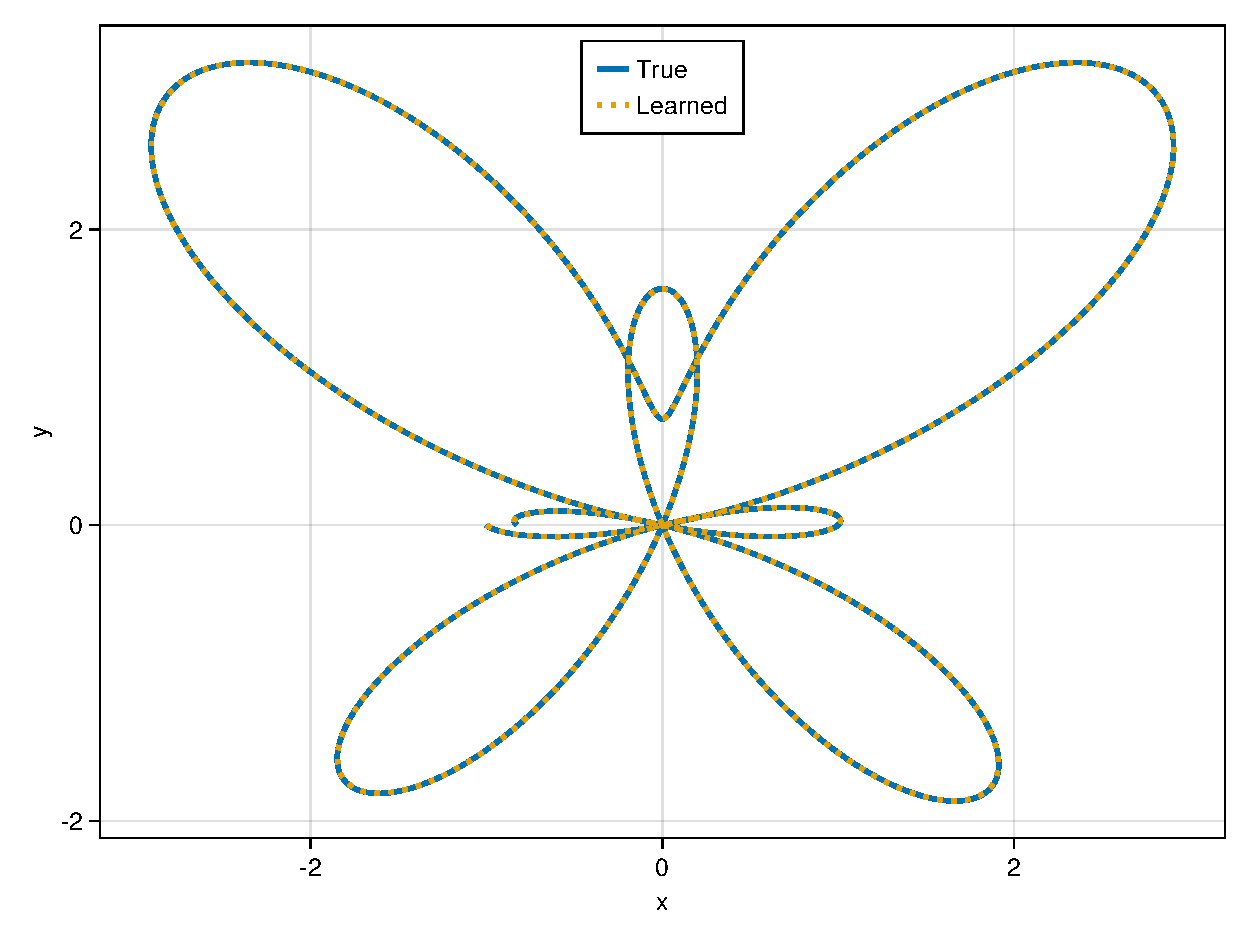
\includegraphics[width=0.8\textwidth]{../figures/lux/cmaes_plot.pdf}
  \caption{CMA-ES optimization to learn the parameters of a neural network that approximates the function $r(\theta) = e^{sin(\theta)} - 2cos(4\theta) + sin\left(\frac{2\theta - \pi}{12}\right)^5$.}
  \label{fig:lux_cmaes_plot}
\end{figure}

\subsection{Physics Informed Neural Networks}
\label{subsec:physics_informed_neural_networks_lux}

In this section, we will describe how to model Physics-Informed Neural Networks (PINNs)~\citep{raissi2019physics} that leverage neural networks to solve Partial Differential Equations~(PDEs). 

% \inputminted[linenos, fontsize=\footnotesize]{julia}{../code/pinn.jl}

NeuralPDEs.jl~\citep{zubov2021neuralpde} extends Lux.jl to provide neural networks solvers for PDEs using PINNs.

% \subsection{Higher Order Taylor Mode Automatic Differentiation}
% \label{subsec:higher_order_taylor_mode_automatic_differentiation}

\section{Leveraging Cross-Language Capabilities}
\label{sec:cross_language_capabilities}

\section{Performance}
\label{sec:performance_lux}

\section{Discussion}
\label{sec:discussion_lux}

\subsection{Current Limitations}
\label{subsec:current_limitations}
